\documentclass[sn-basic]{sn-jnl}

\usepackage{graphicx}
\usepackage{manyfoot}
\usepackage{textcomp}
\usepackage{amsmath,amssymb}
\usepackage{booktabs}
\usepackage{xcolor}
\usepackage{xurl}
\usepackage[title]{appendix}
\graphicspath{{figures/}{../survey/figures/}}
\newcommand{\USD}{US\$}
\newcommand{\INR}{INR~}

\raggedbottom

\begin{document}

\title[FDI and Changing Dimensions of Ownership]{FDI and Changing Dimensions of Ownership: Evidence from India, 2000--2026}

\author*[1]{\fnm{Harsh} \sur{Raj}}\email{applications.harsh@gmail.com}

\affil*[1]{\orgdiv{Department of Finance and Risk Engineering}, \orgname{New York University Tandon School of Engineering}, \orgaddress{\city{Brooklyn}, \state{NY}, \country{USA}}}

\abstract{\textbf{Purpose:} Foreign direct investment (FDI) changes who owns and controls a country's businesses, and its rules are written as limits on ownership. This study examines how FDI into India and the rules on foreign ownership changed between 2000 and 2026, and how employees of multinational companies perceive FDI's effects.
\textbf{Methods:} The study combines official data on gross and net FDI, source countries and sectors from April 2000 to March 2026; a review of sectoral ownership limits and their changes since 1991; and a survey of 100 employees of multinational companies in India, analysed with Wilson intervals, sign tests with Holm adjustment and Fr\'echet bounds on joint agreement.
\textbf{Results:} Gross FDI inflows reached a record \USD 94.8 billion in 2025-26, but repatriation by foreign investors (\USD 53.6 billion) and outward investment by Indian firms (\USD 33.3 billion) left net FDI of \USD 7.7 billion, after it fell to \USD 1.0 billion in 2024-25. Ownership limits rose almost without exception, with insurance moving from 26\% to 100\%, while a 2020 rule made approval depend on the investor's country of origin. About two-thirds of survey respondents agreed with each benefit of FDI and about two-thirds with each concern; at least 46\% agreed both that FDI makes domestic industry more competitive and that it displaces local businesses.
\textbf{Conclusion:} Gross inflows overstate the change in foreign ownership. Ownership now turns over faster, moves back to domestic investors through stock-market sales, and is regulated by who the investor is as well as how much they own.}

\keywords{Foreign direct investment, Ownership structure, Net FDI, Repatriation, Sectoral caps, Press Note 3, India}

\pacs[JEL Classification]{F21, F23, G32, O53}

\maketitle

\section{Introduction}\label{sec:intro}

Foreign direct investment (FDI) is investment by which a foreign company or fund takes a lasting interest in a business, conventionally 10\% or more of its equity. Unlike portfolio investment, which only buys shares, FDI changes who owns and controls companies. For that reason its rules are written as limits on ownership: how much of a sector foreigners may own, whether they need approval, and, since 2020, which countries they may come from.

A foreign company can enter a country by greenfield investment, building a new business under its own ownership; by a joint venture, sharing ownership with a local partner; or by acquisition, buying an existing company in part or in full. Each gives the investor a different degree of control and changes the ownership of the host country's industry in a different way. For much of the period after independence, India kept foreign ownership low: companies with more than 40\% foreign equity were restricted under the Foreign Exchange Regulation Act of 1973. The New Industrial Policy of 1991 allowed automatic approval of up to 51\% foreign ownership in 34 priority industries, and since 2000 most sectors have been open under an automatic route that needs only notification to the Reserve Bank of India (RBI), with the rest requiring government approval and a short list closed altogether. The Foreign Investment Promotion Board, which approved investments case by case, was abolished in 2017.

Three developments have since changed what FDI means for ownership. Private equity, sovereign wealth and pension funds now account for a large share of FDI, and they buy stakes to sell later. Foreign parents have begun to sell stakes in Indian subsidiaries on the Indian stock market, as Hyundai Motor India (\INR 278.7 billion, October 2024) and LG Electronics India (\INR 116 billion, October 2025) did through pure offers for sale \citep{bs2026ipo}. And Indian companies have become foreign owners themselves.

Most discussion of FDI in India focuses on gross inflows, which have risen almost every year. This paper asks how the volume, sources and destinations of FDI into India have changed since 2000; how the limits on foreign ownership have changed; and how people working inside multinational companies see FDI's effect on domestic ownership and industry. It contributes by documenting the widening gap between gross and net FDI since 2023, by tracing the shift from sectoral limits to restrictions based on the investor's origin, and by analysing a survey whose respondents endorse both the benefits and the costs of FDI.

\section{Literature review}\label{sec:lit}

\subsection{Why firms invest abroad}

\citet{hymer1976} argued that a foreign firm starts at a disadvantage against local competitors, so it invests abroad only when it has an advantage of its own, such as technology, a brand or scale, large enough to overcome that handicap; FDI is therefore about control, not just capital. \citet{dunning2000} built this into the eclectic or OLI paradigm, in which a firm invests abroad when ownership advantages, location advantages and internalisation advantages come together. Dunning's investment development path \citep{dunning1981} links a country's net FDI position to its stage of development: as domestic firms build their own ownership advantages, outward investment rises and net FDI moves towards zero. \citet{buckley2009}, reviewing thirty years of internalisation theory, emphasised that the choice between owning and contracting depends on the costs of transacting in imperfect markets for knowledge, and \citet{caves1996} showed how host-country ownership limits push foreign firms into joint ventures they would not otherwise choose.

\subsection{Ownership structure and the host country}

\citet{meyer2011} describe multinationals as embedded both in their global network and in each local context, so that the ownership form they choose reflects how much they need local partners' knowledge and legitimacy. \citet{cantwell2005} show that some subsidiaries create new competences rather than only using the parent's, making technology transfer more likely when subsidiaries are given research mandates. \citet{rugman2004} found that most large multinationals earn most of their sales in their home region, qualifying the idea that FDI makes ownership borderless.

\subsection{Emerging-market multinationals, institutions and distribution}

\citet{ramamurti2012} argued that multinationals from emerging markets such as India compete on cost, on the ability to operate in difficult institutional environments and on acquisitions that buy technology and brands abroad, and \citet{contractor2007} found an S-shaped relationship between international expansion and performance among Indian firms. \citet{cuervo2006} showed that host-country corruption deters FDI, especially from countries that have signed the OECD Anti-Bribery Convention. \citet{helpman2018} finds that trade and FDI have raised inequality within countries, but by less than is often assumed. \citet{unctad2020} documented the collapse of global FDI in the pandemic and the spread of investment screening, of which India's 2020 rule on neighbouring countries is one example.

Most studies of FDI in India measure gross inflows and their links with growth, productivity and exports. The gap between gross and net FDI, large only since 2023, and restrictions based on the investor's country of origin, introduced in 2020, have received little attention; this paper addresses both.

\section{Data and methods}\label{sec:methods}

\subsection{Secondary data}

Financial-year inflows from 2000-01 and cumulative inflows by country and sector are from the Department for Promotion of Industry and Internal Trade (DPIIT) factsheet to June 2025 \citep{dpiit2025}. Inflows by country and sector for 2025-26 are from DPIIT data as reported by \citet{indiabriefing2026}, and total inflows for 2025-26 from the Ministry of Finance \citep{indiatribune2026}. Gross inflows, repatriation, outward investment and net FDI are from RBI data as reported by \citet{bs2024net,bs2025net,bs2026net}. Ownership limits come from DPIIT's consolidated FDI policy and later press notes \citep{dpiit2020}, the insurance amendment of 2025 \citep{pib2025insurance}, the space policy of 2024 and the Cabinet decision of 10 March 2026 \citep{air2026pn3}, cross-checked against \citet{beacon2026}.

\subsection{Survey}

A structured questionnaire of 14 closed statements was answered on a five-point Likert scale (5 strongly agree to 1 strongly disagree) by 100 employees of multinational companies in India at associate, supervisory and higher levels, chosen by convenience sampling. Eight statements describe benefits of FDI, five describe concerns and one asks whether policy should favour attracting FDI over protecting domestic industry (Appendix~\ref{app:q}).

For each statement, the share agreeing (agree or strongly agree) is reported with a 95\% Wilson interval, together with the share disagreeing and the mean score. A two-sided exact sign test compares agreeing with disagreeing answers, leaving out neutral answers, and the $p$-values are adjusted for 14 tests by Holm's method. Only the count of answers for each statement was retained, not each respondent's full set of answers, so answers cannot be correlated across statements. Instead the analysis reports the Fr\'echet lower bound on the share of respondents who agreed with two statements $i$ and $j$ at once:
\begin{equation}
\Pr(A_i \cap A_j) \;\geq\; \max\{0,\ \Pr(A_i) + \Pr(A_j) - 1\},\label{eq:frechet}
\end{equation}
where $A_i$ is the event of agreeing with statement $i$.

\section{Results}\label{sec:results}

\subsection{Inflows since 2000}

FDI into India has grown in four phases (Figure~\ref{fig:inflows}): total inflows below \USD 10 billion a year until 2005-06; a jump to \USD 41.9 billion by 2008-09, following the opening of construction, telecom and retail; a plateau of \USD 34--47 billion until 2013-14; and steady growth from 2014-15 to \USD 84.8 billion in 2021-22, a dip to about \USD 71 billion in 2022-24 as global interest rates rose, and a record \USD 94.8 billion in 2025-26, 18\% more than the year before and 23 times the 2000-01 level \citep{dpiit2025,indiatribune2026}. In 2025-26, 62\% of inflows were new equity (\USD 58.9 billion) and 38\% reinvested earnings and other capital: money foreign-owned companies earned in India and kept there, which raises foreign ownership without new foreign money arriving.

\begin{figure}[t]
\centering
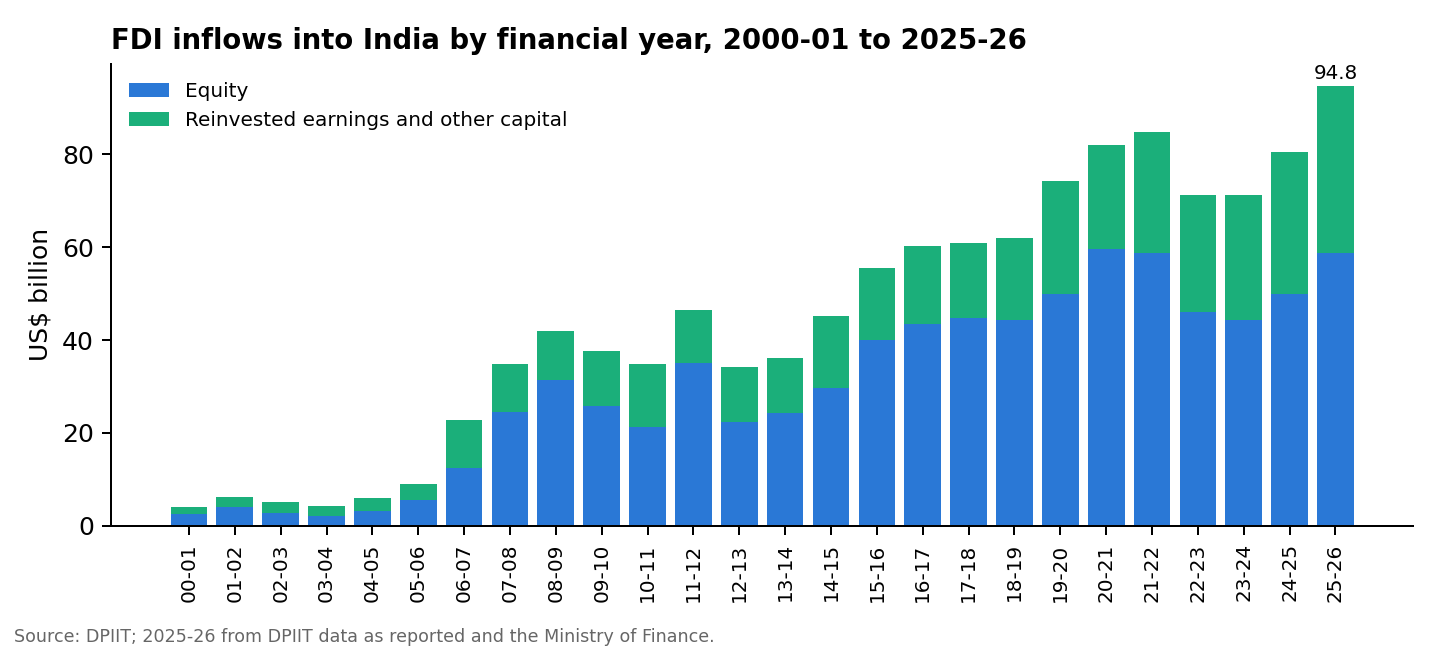
\includegraphics[width=0.95\textwidth]{inflows.png}
\caption{FDI inflows into India by financial year, 2000-01 to 2025-26. Sources: \citet{dpiit2025}; 2025-26 from \citet{indiabriefing2026} and \citet{indiatribune2026}}\label{fig:inflows}
\end{figure}

\subsection{Sources and destinations}

From April 2000 to June 2025, Mauritius (24.4\%) and Singapore (24.0\%) together supplied almost half of equity inflows, followed by the United States (10.2\%), the Netherlands (7.2\%) and Japan (6.0\%) \citep{dpiit2025}. Mauritius and Singapore are mostly conduits: their tax treaties with India made them the natural base for global funds. After the treaties were amended in 2016 to let India tax capital gains on shares bought from April 2017, Mauritius's lead faded; in 2025-26 Singapore supplied 34\% of equity inflows and Mauritius 11\%, while direct investment from the United States doubled from \USD 5.5 billion to \USD 11.2 billion \citep{indiabriefing2026}. Because of this routing, the ultimate owners behind much of India's FDI are not visible in the country data.

Since 2000, services (16.3\%) and computer software and hardware (15.5\%) have received almost a third of equity inflows \citep{dpiit2025}. In 2025-26, software and hardware became the largest destination, at \USD 13.9 billion (24\% of equity), and Maharashtra and Karnataka together received more than half of equity inflows \citep{indiabriefing2026}.

\subsection{Changes in ownership limits}

Table~\ref{tab:timeline} traces the main changes. Three patterns stand out. First, the direction has been almost entirely one way: the only new sectoral cap in the period was on digital news media, set at 26\% in 2019, and insurance shows the typical path of a low initial cap raised step by step (26\% in 2000, 49\% in 2015, 74\% in 2021 and 100\% in 2025 \citep{pib2025insurance}). Second, caps have become tiered, with foreign ownership automatic up to one threshold and subject to approval above it, as in defence (74\% and 100\%), private banks (49\% and 74\%) and launch vehicles (49\% and 100\%). Third, a few sectors remain protected: news media (26\% for print and digital, 49\% for television) and multi-brand retail (51\%, with approval).

The most important change since 2020 is a new dimension of ownership. Press Note 3 of April 2020 made the investor's country of origin, not the sector, the basis for approval: any investment from a country sharing a land border with India, in practice mainly China, needs government approval, and the rule applies to the beneficial owner rather than the immediate investor. In March 2026 the government kept the screening but set a 60-day deadline for decisions \citep{air2026pn3}.

\begin{table}[t]
\caption{Main changes in India's limits on foreign ownership, 1991--2026}\label{tab:timeline}
\footnotesize
\begin{tabular}{@{}lp{3.3cm}p{7.6cm}@{}}
\toprule
Year & Sector & Change \\
\midrule
1991 & All industries & Automatic approval up to 51\% in 34 priority industries \\
2000 & All industries & Automatic route becomes the default; insurance opened at 26\% \\
2012 & Retail & Single-brand retail to 100\%; multi-brand retail opened at 51\% with approval \\
2014 & Defence, railways & Defence from 26\% to 49\%; railway infrastructure 100\% automatic \\
2015 & Insurance & 26\% to 49\% \\
2016 & Defence, aviation, e-commerce & Defence above 49\% with approval; scheduled airlines 49\% automatic and 100\% with approval; e-commerce marketplaces 100\% \\
2017 & All industries & Foreign Investment Promotion Board abolished \\
2018 & Single-brand retail & 100\% automatic \\
2019 & Coal, contract manufacturing, digital media & Coal and contract manufacturing 100\% automatic; digital news media capped at 26\% \\
2020 & Land-border countries & All investment needs government approval (Press Note 3) \\
2020 & Defence & Automatic route from 49\% to 74\% \\
2021 & Insurance, telecom & Insurance 49\% to 74\%; telecom 100\% automatic \\
2024 & Space & Satellites 74\% automatic; launch vehicles 49\% automatic; components 100\% automatic \\
2025 & Insurance & 74\% to 100\% (Act passed 17 December 2025) \\
2026 & Land-border countries & 60-day deadline for approval decisions (10 March 2026) \\
\botrule
\end{tabular}
\footnotetext{Sources: \citet{dpiit2020}, \citet{pib2025insurance}, \citet{air2026pn3}, \citet{beacon2026}.}
\end{table}

\subsection{Gross versus net FDI}

Between 2022-23 and 2025-26, gross inflows rose by a third, but repatriation by foreign investors rose 83\% and outward investment by Indian companies more than doubled (Table~\ref{tab:net}, Figure~\ref{fig:net}). Foreign investors took out 41\% of what came in during 2022-23 and 57\% in 2025-26. Net FDI fell from \USD 28.0 billion to \USD 1.0 billion in 2024-25, the lowest in at least two decades, before recovering to \USD 7.7 billion. Much of the repatriation reflects foreign owners selling stakes built up in earlier years: private equity funds exiting through sales to strategic buyers, and foreign parents selling part of their Indian subsidiaries on the stock market. When a parent sells shares to Indian investors, ownership moves from foreign to domestic hands while the company continues to operate in India; the RBI has described this as the sign of a mature market that investors can enter and leave easily \citep{bs2025net}. The rise in outward investment is consistent with the later stages of Dunning's investment development path. Gross FDI therefore overstates the change in foreign ownership.

\begin{table}[h]
\caption{Gross FDI, money going out and net FDI (\USD billion)}\label{tab:net}
\footnotesize
\begin{tabular}{@{}lrrrr@{}}
\toprule
 & 2022-23 & 2023-24 & 2024-25 & 2025-26 \\
\midrule
Gross FDI inflow & 71.3 & 71.3 & 80.6 & 94.8 \\
Repatriated by foreign investors & 29.3 & 44.5 & 51.5 & 53.6 \\
Invested abroad by Indian firms & 14.0 & 16.7 & 28.2 & 33.3 \\
Net FDI & 28.0 & 10.1 & 1.0 & 7.7 \\
\botrule
\end{tabular}
\footnotetext{Source: RBI data reported by \citet{bs2024net,bs2025net,bs2026net}. Figures are revised between releases, so items may not add exactly.}
\end{table}

\begin{figure}[h]
\centering
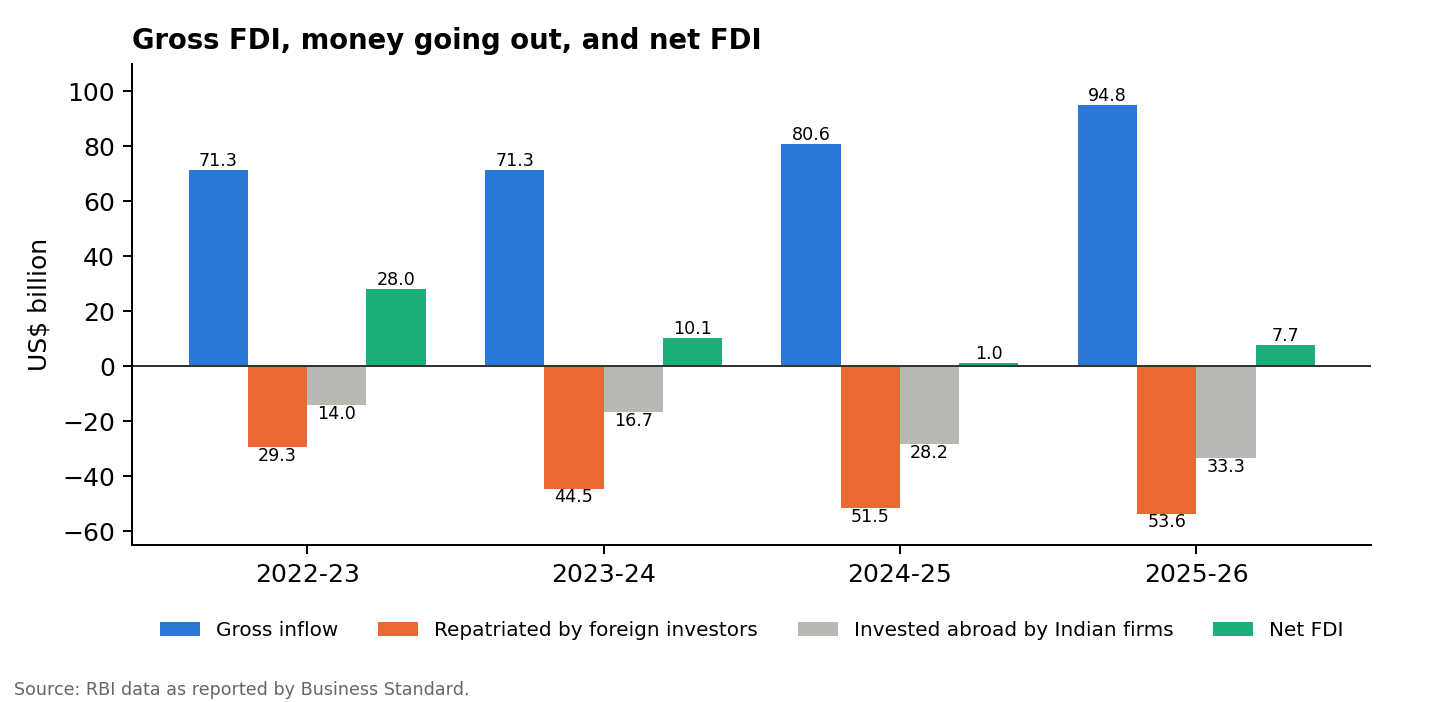
\includegraphics[width=0.95\textwidth]{net.png}
\caption{Gross FDI, repatriation, outward FDI and net FDI, 2022-23 to 2025-26}\label{fig:net}
\end{figure}

\subsection{Survey findings}

Agreement exceeded disagreement for every statement (Table~\ref{tab:survey}, Figure~\ref{fig:likert}; sign test, Holm-adjusted $p \leq 0.003$). Respondents agreed with the benefits and the concerns in equal measure: across the eight benefit statements an average of 67\% agreed, and across the five concern statements also 67\%. The most agreed-with benefit, that FDI encourages partnerships (75\%), was matched exactly by the most agreed-with concern, that FDI displaces local businesses (75\%).

By Eq.~(\ref{eq:frechet}), at least 46\% of respondents agreed both that FDI makes domestic industry more competitive (Q1) and that it displaces local businesses (Q9), and at least 50\% agreed both that it encourages partnerships (Q10) and that it displaces local businesses; every one of the 40 benefit--concern pairs has a lower bound of at least 20\%. These positions are not contradictory, since competition from foreign firms can strengthen an industry while pushing its weaker firms out, but they show that people working inside multinationals do not see FDI as simply good or bad. Views on ownership were likewise mixed: 71\% agreed that FDI diversifies ownership and 67\% that it concentrates ownership in a few multinationals, both of which can hold in different sectors. Two-thirds favoured attracting FDI over protecting domestic industry, consistent with the direction of policy. The weakest agreement concerned resilience (59\%) and sovereignty (61\%), the most abstract statements and the ones with the most disagreement.

\begin{table}[h]
\caption{Survey answers ($n = 100$)}\label{tab:survey}
\footnotesize
\begin{tabular}{@{}llrrrr@{}}
\toprule
 & Statement (short form; full wording in Appendix~\ref{app:q}) & Agree & 95\% interval & Disagree & Mean \\
\midrule
Q10 & Encourages partnerships & 75\% & 66--82\% & 15\% & 3.89 \\
Q9 & Displaces local businesses & 75\% & 66--82\% & 13\% & 3.86 \\
Q1 & Makes domestic industry more competitive & 71\% & 61--79\% & 18\% & 3.79 \\
Q2 & Diversifies ownership & 71\% & 61--79\% & 20\% & 3.75 \\
Q3 & Brings technology and innovation & 71\% & 61--79\% & 19\% & 3.73 \\
Q11 & Loses control of key industries & 70\% & 60--78\% & 22\% & 3.71 \\
Q6 & Concentrates ownership in a few multinationals & 67\% & 57--75\% & 24\% & 3.66 \\
Q7 & Policy should favour FDI over protection & 66\% & 56--75\% & 23\% & 3.66 \\
Q8 & Transfers knowledge and skills & 66\% & 56--75\% & 22\% & 3.66 \\
Q4 & Foreign firms boost growth & 65\% & 55--74\% & 26\% & 3.54 \\
Q5 & Undermines local firms' autonomy & 64\% & 54--73\% & 24\% & 3.59 \\
Q13 & Opens global markets & 61\% & 51--70\% & 25\% & 3.47 \\
Q14 & Undermines national sovereignty & 61\% & 51--70\% & 27\% & 3.37 \\
Q12 & Makes the economy more resilient & 59\% & 49--68\% & 30\% & 3.34 \\
\botrule
\end{tabular}
\footnotetext{Agree: agree or strongly agree, with a 95\% Wilson interval. Mean on a scale of 1 (strongly disagree) to 5 (strongly agree).}
\end{table}

\begin{figure}[h]
\centering
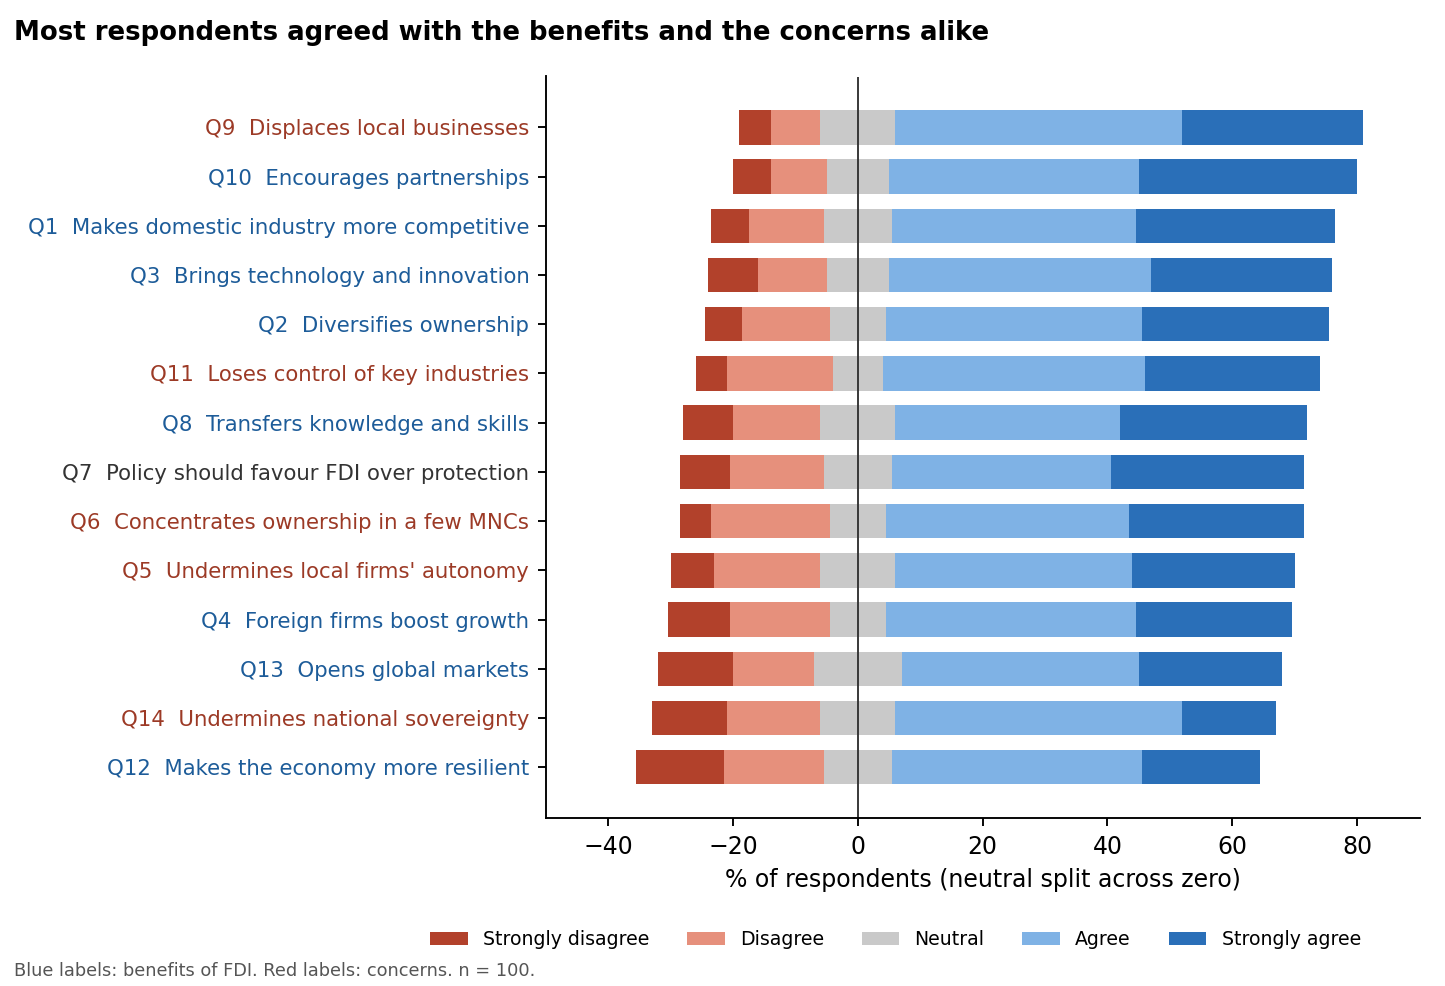
\includegraphics[width=0.9\textwidth]{likert.png}
\caption{Answers to the 14 statements, ordered by net agreement; benefits in blue labels, concerns in red}\label{fig:likert}
\end{figure}

\section{Discussion}\label{sec:discussion}

The results show three ways in which the dimensions of ownership have changed that headline inflows do not reveal. Ownership now turns over: more than half of gross inflows in 2025-26 was offset by repatriation. Foreign owners sell to Indian investors through the stock market, moving ownership back to domestic hands without closing any business. And who the owner is now matters as much as how much they own. The survey reflects this complexity: respondents recognised competition, technology and partnership as benefits while also agreeing that FDI displaces local firms and concentrates control.

For policymakers, the findings suggest tracking net FDI and ownership rather than gross inflows alone, by publishing repatriation and outward investment by sector and country with the quarterly inflow data; keeping liberalisation predictable, as the stepwise opening of insurance has been; applying origin-based screening quickly and transparently, keeping to the 60-day deadline and publishing approval and rejection counts; improving disclosure of ultimate owners, since nearly half of FDI is routed through Mauritius and Singapore; and reviewing the remaining protected sectors on explicit criteria. For businesses, tiered limits make joint ventures and minority stakes the practical route into defence, banking, space and media, and for Indian firms partnerships with foreign investors are the main channel for technology and market access, with control a matter of how the partnership is structured.

The study has limitations. The survey is small, drawn by convenience and limited to employees of multinationals, who may view FDI more favourably than others. Every statement was worded so that agreeing meant holding the stated view, and agreement ranged only from 59\% to 75\%, so part of the pattern may reflect acquiescence; because only answer counts were retained, genuine ambivalence cannot be separated from acquiescence. Country and sector data for 2025-26 come from reports of DPIIT data and may be revised, net FDI figures are revised between releases, and the ownership limits are summarised: many sectors carry further conditions. Future research should collect respondent-level data with reverse-worded statements and a sample including domestic firms, study the effect of foreign-parent share sales on the governance and performance of Indian subsidiaries, and measure how much of India's FDI is ultimately owned by residents of third countries or of India itself.

\section{Conclusion}\label{sec:conclusion}

In the quarter-century since 2000, FDI into India has grown from \USD 4 billion a year to a record \USD 94.8 billion, and the rules on foreign ownership have opened sector by sector, almost always in one direction. Yet gross inflows overstate the change in foreign ownership: repatriation and outward investment have risen faster, net FDI has fallen to a fraction of gross inflows, and since 2020 the investor's origin has become a dimension of ownership in its own right. FDI is therefore not simply a matter of attracting more foreign capital. It changes who owns the economy, and that change needs to be measured and managed.

\backmatter

\bmhead{Acknowledgements}
The author thanks the employees who took part in the survey.

\section*{Declarations}

\begin{itemize}
\item \textbf{Funding:} No funding was received for this study.
\item \textbf{Competing interests:} The author has no competing interests to declare.
\item \textbf{Ethics approval and consent to participate:} Participation in the survey was voluntary, and only aggregate answer counts were retained; no personal identifying information is reported.
\item \textbf{Data availability:} All data used in this study, including the survey answer counts, are available at \url{https://github.com/harsh-github007/FDI-and-Changing-Dimensions-of-Ownership}.
\item \textbf{Code availability:} The survey analysis and figure scripts are available in the same repository, and the data can be explored at \url{https://harsh-github007.github.io/FDI-and-Changing-Dimensions-of-Ownership/}.
\item \textbf{Author contributions:} Harsh Raj designed the study, collected and analysed the data and wrote the manuscript.
\end{itemize}

\begin{appendices}

\section{Questionnaire}\label{app:q}

Respondents rated each statement from 5 (strongly agree) to 1 (strongly disagree).

\begin{enumerate}
\item FDI enhances the competitiveness of domestic industries.
\item FDI leads to a more diversified ownership structure in domestic markets.
\item FDI contributes to technological advancements and innovation in domestic industries.
\item The involvement of foreign-owned companies in domestic markets positively impacts overall economic growth.
\item FDI undermines the autonomy of local businesses.
\item FDI leads to the concentration of ownership in the hands of a few multinational corporations.
\item Government policies should prioritize attracting FDI over protecting domestic industries.
\item FDI fosters knowledge transfer and skill development within domestic workforce.
\item The rise of FDI results in the displacement of local businesses.
\item FDI encourages collaboration and partnership between domestic and foreign entities.
\item FDI leads to a loss of control over key industries within a country.
\item FDI promotes economic diversification and resilience in domestic markets.
\item FDI facilitates access to global markets for domestic businesses.
\item FDI undermines national sovereignty by allowing foreign entities to exert influence over local economies.
\end{enumerate}

\end{appendices}

\bibliography{references}

\end{document}
